\documentclass{article}
\usepackage[utf8]{inputenc}
\usepackage{tikz}
\usepackage{tikz-cd}
\usepackage{graphicx} % Required for inserting images
\usepackage[a4paper, margin=1in]{geometry}
\usepackage{amsfonts}
\usepackage{amsmath} % Set custom margins
\usepackage{parskip}
\usepackage{amssymb} % disable indentation
\usepackage{amsthm}
\usepackage{annotate-equations}
\usetikzlibrary{decorations.pathreplacing}


\title{Category Theory - Lecture 4 (Notes)}
\author{Vorashil Farzaliyev}
\date{September 2024}

\newtheorem{remark}{Remark}[section]
\newtheorem{lemma}{Lemma}[section]
\newtheorem{proposition}{Proposition}[section]
\newtheorem{definition}{Definition}[section]
\newtheorem{observation}{Observation}[section]
\newtheorem{example}{Example}[section]
\newtheorem{exercise}{Exercise}[section]
\newtheorem{theorem}{Theorem}[section]
\newtheorem{note}{Note}[section]

\renewcommand{\shorto}{\to}
% new command for making \mapsto 0.5cm

\renewcommand{\to}{\xrightarrow{\hspace{0.5cm}}}  % Adjust the length as needed
\renewcommand{\mapsto}{\mathrel{\kernel\longmapsto\kernel}}  % Adjust spacing with \mkern if needed

\begin{document}
    \maketitle


    \section{Surjective functors}

    \[
        \begin{array}{rl}
            \parbox{6cm}{ % Adjust width to fit the text properly
                Write $A \cong B$ to mean that $A$ and $B$ are isomorphic,\\
                i.e., $f: A \to B$ is an isomorphism.
            } &
            \hspace{2cm} % Adds space between the text and the diagram
            \begin{tikzpicture}
                [baseline={(current bounding box.center)}, scale=2] % Increased scale to make the diagram bigger
                % Draw the circle
                \draw[thick] (1.5, 1) circle (1.5);  % Circle centered at (1.5, 1) with radius 1

                % Place the points inside the circle
                \filldraw (1.5, 1.7) circle (1pt)
                \node at (1.5, 1.85) {A};  % Top point
                \filldraw (0.7, 1) circle (1pt)
                \node at (0.7, 1.2) {D};    % Left point
                \filldraw (2.3, 1) circle (1pt)
                \node at (2.3, 1.2) {B};    % Right point
                \filldraw (1.5, 0.2) circle (1pt)
                \node at (1.5, 0.05) {C};  % Bottom point

                % Draw straight arrows between the points
                \draw[->] (1.5, 1.7) -- (2.2, 1.1);  % Arrow from A to B
                \draw[->] (0.72, 0.9) -- (1.3, 0.3);    % Arrow from D to C

                % Draw curved arrows
                \draw[->, bend right] (0.65, 0.9) to (1.4, 0.2);  % Curved arrow from D to C
                \draw[->, bend left] (0.75, 1) to (1.5, 0.3);  % Curved arrow from D to C
                \draw[->, bend right] (2.2, 0.9) to (1.55, 0.3); % Curved arrow from B to C
                \draw[->, bend left] (2.4, 0.9) to (1.6, 0.2); % Curved arrow from B to C

            \end{tikzpicture}
        \end{array}
    \]

    \begin{definition}(Surjective functor)
        Let F: \(\mathbf{C} \to \mathbf{D}\) be a functor.

        We say that \(F\) is \textbf{essentially surjective} if for all \(X \in \mathbf{D}\), there exists a \(A\) such that \(F(A) \cong X\).

        \[
            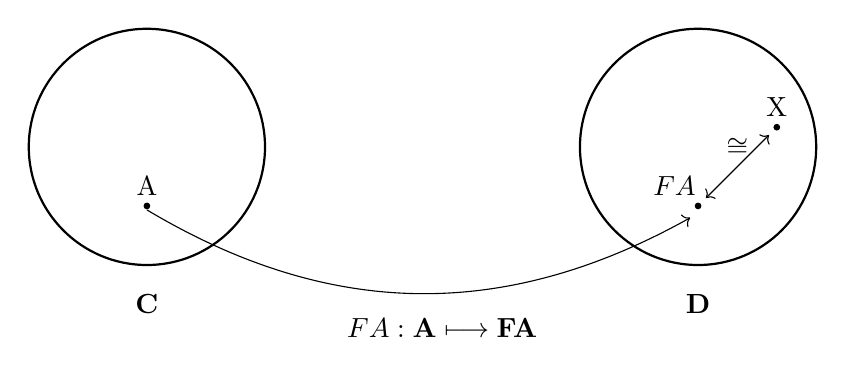
\begin{tikzpicture}
                % Draw the first circle
                \draw[thick] (0,0) circle (1.5);  % Circle centered at (0, 0) with radius 1
                \filldraw (0, -0.75) circle (1pt);  % Visible dot for point A
                \node at (0, -0.5) {A};  % Label for point A
                \node at (0, -2) {$\mathbf{C}$};  % Label for the functor

                % Draw the second circle
                \draw[thick] (7,0) circle (1.5);  % Circle centered at (4, 0) with radius 1
                \filldraw (8, 0.25) circle (1pt);  % Visible dot for point B
                \node at (8, 0.5) {X};  % Top point in the second circle
                \filldraw (7, -0.75) circle (1pt);  % Visible dot for point C
                \node at (6.7, -0.5) {$FA$};  % Bottom point in the second circle
                \node at (3.75, -2.3) {$FA: \mathbf{A} \mapsto \mathbf{FA}$};  % Label for the functor
                \node at (7, -2) {$\mathbf{D}$};  % Label for the functor

                % Draw the connecting line from the point A to point C (bottom-most in second circle)
                \draw[->, bend right] (0, -0.8) to (6.9, -0.9);  % Line from A to C
                % Draw the line from B to C with the isomorphism symbol
                \draw[<->] (7.9, 0.15) -- (7.1, -0.65)
                node[midway, above] {$\cong$};  % Line from B to C with \cong in the middle
            \end{tikzpicture}
        \]


    \end{definition}

    \vspace{0.2in}

    \newpage

    \begin{example}
        Let \(F: \mathbf{C} \to \mathbf{D}\) be a functor.

        \newline

        \begin{itemize}
            \item For \(\mathbf{C}\) =
            \[
                \mathbf{C} = \text{ category of }
                \left\{
                \begin{array}{ll}
                [n]
                    = \{1, 2, \dots, n\} \text{ for } n \in \mathbb{N} \} \\
                    \vspace{0.1in}                                        \\
                    \text{$[n]$} \stackrel{f}{\to} \text{$[m]$}           \\
                \end{array}
                \right.
            \]
            \item For \(\mathbf{D}\) = \underline{FinSet}
            \[
                \underline{FinSet} = \text{ category of }
                \left\{
                \begin{array}{ll}
                    \text{finite sets} \\
                    \vspace{0.1in}     \\
                    \text{functions}   \\
                \end{array}
                \right.
            \]
        \end{itemize}

        \[
            \begin{tikzcd}[column sep=4em, row sep=4em]
            [n]
                \arrow[r, "F"] \arrow[d, "f"]
                & \{1, 2, \dots, n\} \arrow[d, "Ff=f"] \\
                \text{$[m]$} \arrow[r, "F"]
                & \{1, 2, \dots, m\}
            \end{tikzcd}
        \]

        For example, \(\{1, 3\} \in \underline{FinSet}\)  is not in the (essential) image of \(F\).
        However, we have \([2] \in \mathbf{C}\) and
        \[
            F([2]) \cong \{1, 3\} \in \underline{FinSet}
        \]
    \end{example}


    \section{Full and Faithful Functors}

    \begin{definition} (Faithful functor)

        Let \(F: \mathbf{C} \to \mathbf{D}\) be a functor. We say that \(F\) is \textbf{faithful} if \(\forall A, B \in \mathbf{C}\) the function
        \[
            \mathbf{C}(A, B) \to \mathbf{D}(F(A), F(B))
        \]
        is injective.

    \end{definition}

    \begin{definition} (Full functor)

        Let \(F: \mathbf{C} \to \mathbf{D}\) be a functor. We say that \(F\) is \textbf{full} if \(\forall A, B \in \mathbf{C}\) the function
        \[
            \mathbf{C}(A, B) \to \mathbf{D}(F(A), F(B))
        \]
        is surjective.
    \end{definition}

    \begin{note} (What does it mean for a functor to be full?)

        For all \(A, B \in \mathbf{C}\), we have
        \[
            \mathbf{C}(A, B) \to \mathbf{D}(F(A), F(B)) \text{ is surjective}
        \]
        means \(\forall u: FA \to FB\) in \(\mathbf{D}\) there exists \(f: A \to B\) in \(\mathbf{C}\) such that
        \[
            Ff = u
        \]

    \end{note}

    \begin{note} (What does it mean for a functor to be faithful?)

        For all \(A, B \in \mathbf{C}\), we have
        \[
            \mathbf{C}(A, B) \to \mathbf{D}(F(A), F(B)) \text{ is injective}
        \]
        means \(\forall f_1, f_2: A \to B\) in \(\mathbf{C}\)
        \[
            F(f_1) = F(f_2) \Rightarrow f_1 = f_2
        \]
    \end{note}

    \subsection{Examples}

    \begin{example} (\(F: \underline{Grp} \to \underline{Set}\))
        \[
            \underline{Grp} \to \underline{Set}
        \]
        \[
            \begin{tikzcd}[column sep=4em, row sep=4em]
            (G, \circ)
                \arrow[r, "F"] \arrow[d, "f"]
                & G = F(G, \circ) \arrow[d, "Ff=f"] \\
                (H, *) \arrow[r, "F"]
                & H = F(H, *)
            \end{tikzcd}
        \]
        So we have
        \begin{gather*}
            \underline{Grp}((G, \circ), (H, *)) \mapsto \underline{Set}(G, H)\\
            f \mapsto f\\
        \end{gather*}
        not full, but faithful.

        \begin{itemize}
            \item \textbf{not full}: Because a map in $\underline{Grp}$ is a group homomorphism, but not every map
            in $\underline{Set}$ corresponds to a group homomorphism. So we can fund
            \(u: G \to H\) in $\underline{Set}$ such that there is no \(f: (G, \circ) \to (H, *)\) in $\underline{Grp}$ such that \(Ff = u\).
            \item \textbf{faithful}: since it injectively maps every map \(f: G \to H\) in $\underline{Grp}$ to a map \(Ff: GF \to FH\) in $\underline{Set}$.
        \end{itemize}

    \end{example}

    \begin{example} (\(F: \underline{Ab} \to \underline{Grp}\))
        \[
            \underline{Ab} \to \underline{Grp}
        \]
        \[
            \begin{tikzcd}[column sep=4em, row sep=4em]
            (G, \circ)
                \arrow[r, "F"] \arrow[d, "f"]
                & (G, \circ) = F(G, \circ) \arrow[d, "Ff=f"] \\
                (H, *) \arrow[r, "F"]
                & (H, *) = F(H, *)
            \end{tikzcd}
        \]
        So we have
        \begin{gather*}
            \underline{Grp}((G, \circ), (H, *)) \mapsto \underline{Set}(G, H)\\
            f \mapsto f\\
        \end{gather*}
        full and faithful.

        \begin{itemize}
            \item \textbf{full}: every group homomorphism between \( F(G, \circ) \) and \( F(H, *) \) comes from an abelian group homomorphism between \( (G, \circ) \) and \( (H, *) \).
            \item \textbf{faithful}: $F$ is faithful because it injectively maps abelian group homomorphisms to group homomorphisms
        \end{itemize}
    \end{example}

    \begin{exercise}
        Find a functor \(F: \mathbf{C} \to \mathbf{D}\) that is full but not faithful.

        \begin{itemize}
            \item think small categories
            \item \(\underline{P} \to \underline{Q}\)
        \end{itemize}
    \end{exercise}

    \newpage


    \section{Subcategories}


    \begin{definition}
        Let \(\mathbf{C}\) be a category.

        A \textbf{subcategory} \(\mathbf{D}\) of \(\mathbf{C}\)  consists of

        \begin{itemize}
            \item a subclass
            \[
                Ob(\mathbf{D}) \subseteq Ob(\mathbf{C})
            \]
            \item \(\forall A, B \in Ob(\mathbf{D}) \subseteq Ob(\mathbf{C})\)
            \[
                \mathbf{D}(A, B) \subseteq \mathbf{C}(A, B)
            \]
        \end{itemize}
        which is closed under composition and identities:
        \begin{itemize}
            \item \(\forall A, B, C \in Ob(\mathbf{D})\)
            \vspace{0.1in}
            \[
                f \in \mathbf{D}(A, B) \) \text{ and } g \in \mathbf{D}(B, C)  \Rightarrow \( g \circ f \in \mathbf{D}(A, C) \)
            \]
%            \vspace{0.2in}
            \item \(\forall A \in Ob(\mathbf{D})\)
            \vspace{0.1in}

            \[
                1_A \in \mathbf{D}(A, A)
            \]
        \end{itemize}
    \end{definition}

    \vspace{0.2in}

    \begin{definition}
        Let \(\mathbf{C}\) be a category and \(\mathbf{D}\) be a subcategory of \(\mathbf{C}\).

        We say that \(\mathbf{D}\) is \textbf{full} if
        \[
            \mathbf{D}(A, B) = \mathbf{C}(A, B)
        \]
        for all \(A, B \in Ob(\mathbf{D})\).
    \end{definition}

    \vspace{0.2in}

    \begin{example} (Subcategories of \(\underline{Set}\))
        \begin{itemize}
            \item \(\underline{Finset} \subseteq \underline{Set}\) is full subcategory of
            \(\underline{Set}\) with objects as finite sets
            \item \(\underline{Finset}_{i,j} \subseteq \underline{Set}\), the subcategory of
            \(\underline{Set}\) with objects finite sets and bijections between them
        \end{itemize}
    \end{example}

    \vspace{0.2in}

    \begin{exercise}


        Let \(G\) be a group.
        Describe explicitly in terms of \(G\), what is the subcategory of \(\Sigma(G)\).

    \end{exercise}

    \begin{exercise}
        Let \(\underline{P}\) be a poset. Describe explicitly in terms of \(\underline{P}\), what is the subcategory of \(\underline{P}\).
    \end{exercise}

\end{document}
